% This contents of this file will be inserted into the _Solutions version of the
% output tex document.  Here's an example:

% If assignment with subquestion (1.a) requires a written response, you will
% find the following flag within this document: <SCPD_SUBMISSION_TAG>_1a
% In this example, you would insert the LaTeX for your solution to (1.a) between
% the <SCPD_SUBMISSION_TAG>_1a flags.  If you also constrain your answer between the
% START_CODE_HERE and END_CODE_HERE flags, your LaTeX will be styled as a
% solution within the final document.

% Please do not use the '<SCPD_SUBMISSION_TAG>' character anywhere within your code.  As expected,
% that will confuse the regular expressions we use to identify your solution.

\def\assignmentnum{4 }
% \def\assignmentname{Sentiment Analysis}
\def\assignmenttitle{XCS234 Assignment \assignmentnum}
\input{macros}
\begin{document}
\pagestyle{myheadings} \markboth{}{\assignmenttitle}

% <SCPD_SUBMISSION_TAG>_entire_submission

This handout includes space for every question that requires a written response.
Please feel free to use it to handwrite your solutions (legibly, please).  If
you choose to typeset your solutions, the |README.md| for this assignment includes
instructions to regenerate this handout with your typeset \LaTeX{} solutions.
\ruleskip

\LARGE
1.a
\normalsize

% <SCPD_SUBMISSION_TAG>_1a
\begin{answer}
  % ### START CODE HERE ###
  It's generally very difficult to translate high level objectives
  into a math mathematical reward function an agent can optimize and
  it is very difficult to avoid reward hacking that results in an
  unintended consequences.

  Example: Content recommendation agent

  The reward function could be number of clicks. The unintended result
  could be recommending all the clickbait contents instead of high quality,
  actually interesting contents.
  % ### END CODE HERE ###
\end{answer}
% <SCPD_SUBMISSION_TAG>_1a
\clearpage

\LARGE
1.b
\normalsize

% <SCPD_SUBMISSION_TAG>_1b
\begin{answer}
  % ### START CODE HERE ###
  It's a single legged robot trying to hop forward.

  \begin{align*}
    \text{reward} = \text{healthy\_reward} + \text{forward\_reward} - \text{ctrl\_cost}
  \end{align*}

  Where

  \begin{align*}
    \text{healthy\_reward}&: \text{Keep the agent to stand by keeping the torso in a healthy state} \\
    \text{forward\_reward}&: \text{Push the agent to move forward by maximize the x-velocity} \\
    \text{ctrl\_cost}&: \text{Prevent the agent to aggressively move, i.e. move smoothly by penalize the large control}
  \end{align*}
  % ### END CODE HERE ###
\end{answer}
% <SCPD_SUBMISSION_TAG>_1b
\clearpage


\LARGE
1.c
\normalsize

% <SCPD_SUBMISSION_TAG>_1c
\begin{answer}
  % ### START CODE HERE ###
  It means the hopper is standing and not falling over. It is
  determine by two factors: the torso's height must be above
  0.8 meters, and its angle must be within 0.2 radians of vertical.

  Advantage of early-termination: speed up training.

  Disadvantage of early-termination: can't learn to recover from falling.
  % ### END CODE HERE ###
\end{answer}
% <SCPD_SUBMISSION_TAG>_1c
\clearpage


\LARGE
1.e
\normalsize

% <SCPD_SUBMISSION_TAG>_1e
\begin{answer}
  % ### START CODE HERE ###
  \begin{figure}[H]
  \centering
    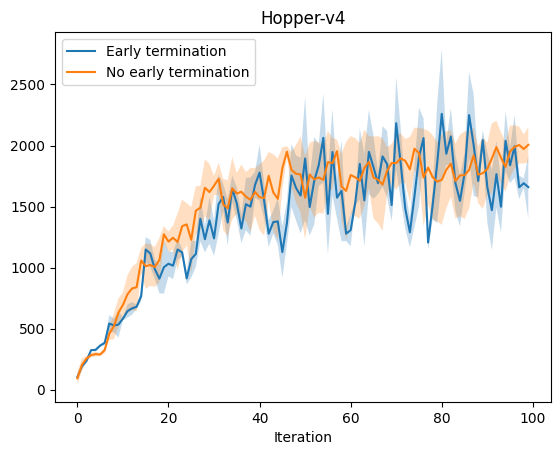
\includegraphics[width=.5\linewidth]{images/ppo_hopper_submission.png}
  \end{figure}
  The performance without early-termination is better than with
  early-termination. It also more consistent, i.e. the standard error
  is smaller. To get better estimate, we should sample more times
  by using different random seeds (at least 10-20 times).
  % ### END CODE HERE ###
\end{answer}
% <SCPD_SUBMISSION_TAG>_1e
\clearpage

\LARGE
1.f
\normalsize

% <SCPD_SUBMISSION_TAG>_1f
\begin{answer}
  % ### START CODE HERE ###
  I looked at a rendered video of the agent trained without early-termination.

  The agent seem to learn some basic control an able to move forward.
  But it also keep repeatedly falling and trying to stand up again.

  It partially complete the task because it's moving. But it fails to keep
  the agent in a healthy state. It doesn't seem to be too surprised because
  the reward function doesn't care about the continuous time it keep
  in the healthy state.
  % ### END CODE HERE ###
\end{answer}
% <SCPD_SUBMISSION_TAG>_1f
\clearpage


\LARGE
1.g
\normalsize

% <SCPD_SUBMISSION_TAG>_1g
\begin{answer}
  % ### START CODE HERE ###
  I looked at another without-early-termination model.

  The agent quickly falling over with very little progress. It still
  able to crawling forward on the ground but never stand up again.
  I would consider this a completely failing.
  % ### END CODE HERE ###
\end{answer}
% <SCPD_SUBMISSION_TAG>_1g
\clearpage

\LARGE
2.a
\normalsize

% <SCPD_SUBMISSION_TAG>_2a
\begin{answer}
  % ### START CODE HERE ###
  Let $R_1 = \sum \hat{r}(o^1, a^1) = \sum \phi_w(o^1, a^1)$
  and $R_2 = \sum \hat{r}(o^2, a^2) = \sum \phi_w(o^2, a^2)$.

  We can express the Bradley-Terry in sigmoid form.
  \begin{align*}
    \hat{P}[\sigma^1 > \sigma^2] &= \frac{e^{R1}}{e^{R1} + e^{R2}} \\
      &= \frac{1}{1 + e^{-(R1 - R2)}} \\
      &= \sigma(R_1 - R_2)
  \end{align*}

  Substitute into loss function
  \begin{align*}
    L = - \left( \mu(1) \log(\sigma(R_1 - R_2)) + \mu(2) \log(\sigma(R_2 - R_1)) \right)
  \end{align*}

  Let $z = R_1 - R_2$, applying chain rule
  \begin{align*}
    \nabla_w L &= [-\mu(1)(1-\sigma(z)) + \mu(2)\sigma(z)] \nabla_w z \\
    &= [-\mu(1) + \mu(1)\sigma(z) + \mu(2)\sigma(z)] \nabla_w z \\
    &= [(\mu(1) + \mu(2))\sigma(z) - \mu(1)] \nabla_w z \\
    &= [(\mu(1) + \mu(2))\sigma(R_1 - R_2) - \mu(1)] \nabla_w(R_1 - R_2) \\
    &= [(\mu(1) + \mu(2))\sigma(\sum_t \phi_w(o_t^1, a_t^1) - \sum_t \phi_w(o_t^2, a_t^2)) - \mu(1)] (\sum_t \nabla_w \phi_w(o_t^1, a_t^1) - \sum_t \nabla_w \phi_w(o_t^2, a_t^2))
  \end{align*}
  % ### END CODE HERE ###
\end{answer}
% <SCPD_SUBMISSION_TAG>_2a
\clearpage

\LARGE
2.b
\normalsize

% <SCPD_SUBMISSION_TAG>_2b
\begin{answer}
  % ### START CODE HERE ###
  I got the following pairs

  3147 (equally preferred): agree, no obvious differences
  % ### END CODE HERE ###
\end{answer}
% <SCPD_SUBMISSION_TAG>_2b
\clearpage

\LARGE
2.c
\normalsize

% <SCPD_SUBMISSION_TAG>_2c
\begin{answer}
  % ### START CODE HERE ###
  Four more pairs:

  4191 (equally preferred): agree, no obvious differences

  6599 (one is preferred): not agree, the non-preferred one has better ending ankle angle to land

  6844 (one is preferred): similar to 6599

  7324 (one is preferred): agree, the preferred one landed on its heel, which is a better position to initiate the next hop

  I am not confident to say I trust this data because firstly the sample is very short, and I disagree some of the samples.
  % ### END CODE HERE ###
\end{answer}
% <SCPD_SUBMISSION_TAG>_2c
\clearpage

\LARGE
2.e
\normalsize

% <SCPD_SUBMISSION_TAG>_2e
\begin{answer}
  % ### START CODE HERE ###
  \begin{figure}[H]
  \centering
    
\includegraphics[width=.5\linewidth]{images/hopper_rlhf.png}
  \end{figure}
  They are highly correlated.
  % ### END CODE HERE ###
\end{answer}
% <SCPD_SUBMISSION_TAG>_2e
\clearpage

\LARGE
2.f
\normalsize

% <SCPD_SUBMISSION_TAG>_2f
\begin{answer}
  % ### START CODE HERE ###
  It does not identifiable because it has very similar trend as the original reward.
  % ### END CODE HERE ###
\end{answer}
% <SCPD_SUBMISSION_TAG>_2f
\clearpage


\LARGE
2.g
\normalsize

% <SCPD_SUBMISSION_TAG>_2g
\begin{answer}
  % ### START CODE HERE ###
  It can perform more hops but fall and never get up again.
  I think it is better in terms of hopping but the original
  policies can move forward more. Can't say which one is better
  but the RLHF seems working as we prefer a landing position
  that is easier to initiate next hop.
  % ### END CODE HERE ###
\end{answer}
% <SCPD_SUBMISSION_TAG>_2g
\clearpage

\LARGE
3.d
\normalsize

% <SCPD_SUBMISSION_TAG>_3d
\begin{answer}
  % ### START CODE HERE ###
  \begin{figure}[H]
  \centering
    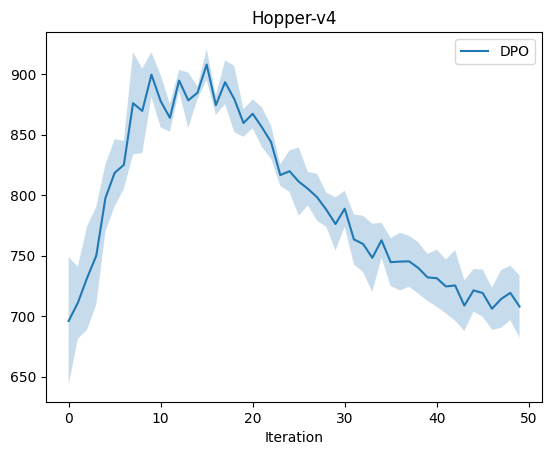
\includegraphics[width=.5\linewidth]{images/hopper_dpo.png}
  \end{figure}
  The DPO reaches max reward of 950, which better than RLHF
  but it degraded after it reaches the peak, suggesting overfitting.

  Pros and Cons
  \begin{center}
  \begin{tabular}{|c c c|}
  \hline
  \thead{Method} & \thead{Pros} & \thead{Cons} \\
  \hline
  RLHF & \makecell{More intuitive as it has a two-staged structure.}
       & \makecell{Unstable. The error in the reward function can be \\
                   exaggerated by the RL algorithm.}  \\
  DPO & \makecell{Avoiding a separate reward function. \\
                  The RL algorithm can directly optimize the policy.}
      & May overfit the preference data. \\
  \hline
  \end{tabular}
  \end{center}
  % ### END CODE HERE ###
\end{answer}
% <SCPD_SUBMISSION_TAG>_3d
\clearpage

\LARGE
3.e
\normalsize

% <SCPD_SUBMISSION_TAG>_3e
\begin{answer}
  % ### START CODE HERE ###
  To be honest, I don't see significant differences. DPO doesn't seem to improve the performance.
  % ### END CODE HERE ###
\end{answer}
% <SCPD_SUBMISSION_TAG>_3e
\clearpage

\LARGE
4.a
\normalsize

% <SCPD_SUBMISSION_TAG>_4a
\begin{answer}
  % ### START CODE HERE ###
  The raters are often contract worker or from a crowdsourcing
  platform. These worker typically are from a low-income background.
  If the raters are not diverse enough, the model may has strong bias
  on some sensitive topics.
  % ### END CODE HERE ###
\end{answer}
% <SCPD_SUBMISSION_TAG>_4a
\clearpage

\LARGE
4.b
\normalsize

% <SCPD_SUBMISSION_TAG>_4b
\begin{answer}
  % ### START CODE HERE ###
  No, the medical diagnoses is strongly rely on domain
  knowledge and must be objective. It shouldn't rely on
  preferences. Unless the model has acceptable level of
  correctness, the RLHF may be used to improve the way
  it structure the response.
  % ### END CODE HERE ###
\end{answer}
% <SCPD_SUBMISSION_TAG>_4b
\clearpage

\LARGE
4.c
\normalsize

% <SCPD_SUBMISSION_TAG>_4c
\begin{answer}
  % ### START CODE HERE ###
  RLHF is lack of factuality checks. Human raters may be
  lack of specific domain knowledge to do factuality checks
  and prefer answers that is well-written or easier to read,
  even if they are inaccurate.
  % ### END CODE HERE ###
\end{answer}
% <SCPD_SUBMISSION_TAG>_4c
\clearpage


% <SCPD_SUBMISSION_TAG>_entire_submission

\end{document}
